\documentclass[10pt, border=10pt]{standalone}
\input{../../tikzpic_packages.tex}

\def\pneumaticcolor{blue!20}

\begin{document}

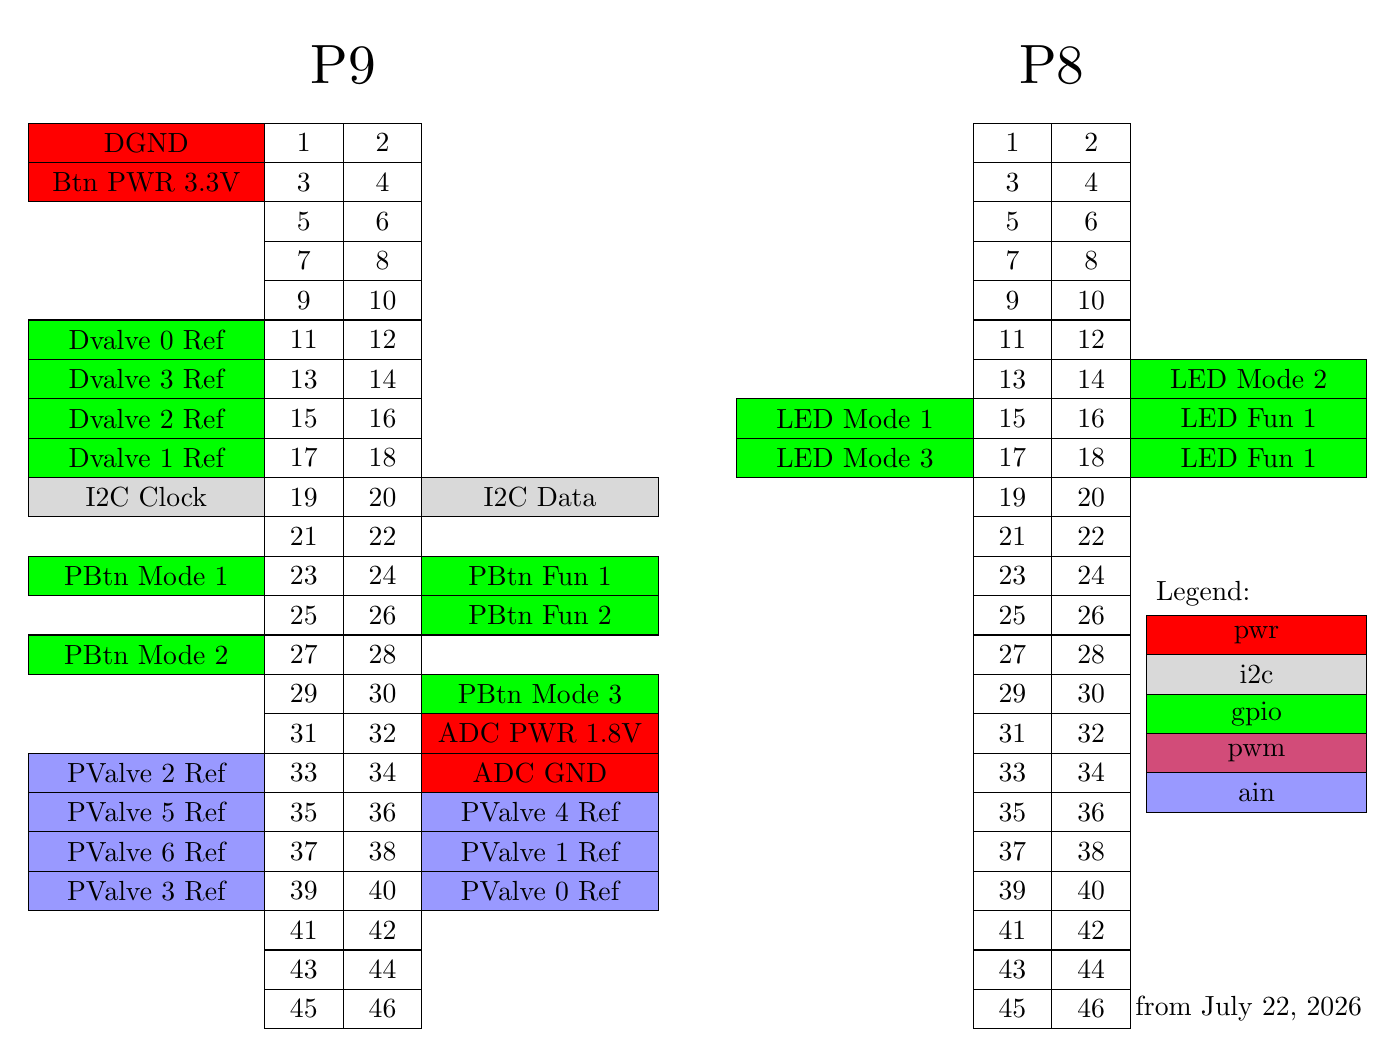
\begin{tikzpicture}[
gpio/.style={fill=green},
ain/.style={fill=blue!40},
pwm/.style={fill=purple!70},
pwr/.style={fill=red},
i2c/.style={fill=gray!30},
pins/.style={midway},
fun/.style={midway, black},
stats/.style={draw=none}
]

\def\w{3}
\def\ws{1}
\def\h{.5}



%%% P9
\path (0,0) coordinate(O)++(\ws,\h)node[above, scale=2]{P9};
\foreach \i in {1,...,46}{
	\pgfmathsetmacro{\shift}{mod(\i-1,2)*\ws}
	\pgfmathsetmacro{\y}{(\i-\shift)*.5*\h}
	\ifodd\i
		\path (O)++(\shift,-\y)coordinate(\i);
	\else
		\path (O)++(\shift+\ws,-\y)coordinate(\i); \fi
	\draw (O)++(\shift,-\y)rectangle++(\ws,\h)node[pins]{\i};
}

\foreach \pin/\fun/\txt in {
	11/gpio/Dvalve 0 Ref,
	13/gpio/Dvalve 3 Ref,
	15/gpio/Dvalve 2 Ref,
	17/gpio/Dvalve 1 Ref,
	23/gpio/PBtn Mode 1,
	27/gpio/PBtn Mode 2,
	30/gpio/PBtn Mode 3,
	24/gpio/PBtn Fun 1,
	26/gpio/PBtn Fun 2,
%	14/pwm/PValve 4 Signal,
%	16/pwm/PValve 5 Signal,
%	21/pwm/PValve 2 Signal,
%	22/pwm/PValve 0 Signal,
%	28/pwm/PValve 6 Signal,
%	42/pwm/PValve 7 Signal,
	19/i2c/I2C Clock,
	20/i2c/I2C Data,
	33/ain/PValve 2 Ref,
	35/ain/PValve 5 Ref,
	37/ain/PValve 6 Ref,
	39/ain/PValve 3 Ref,
	36/ain/PValve 4 Ref,
	38/ain/PValve 1 Ref,
	40/ain/PValve 0 Ref,
	3/pwr/Btn PWR 3.3V,
%	5/pwr/Sens PWR 5V,
	1/pwr/DGND,
	32/pwr/ADC PWR 1.8V,
	34/pwr/ADC GND
	}{
	\ifodd\pin
		\draw[\fun](\pin)rectangle++(-\w,\h)node[fun]{\txt};
	\else
		\draw[\fun](\pin)rectangle++(\w,\h)node[fun]{\txt}; \fi
	}



%%% P8
\path (\w+\w+\w,0) coordinate(O)++(\ws,\h)node[above, scale=2]{P8};
\foreach \i in {1,...,46}{
	\pgfmathsetmacro{\shift}{mod(\i-1,2)*\ws}
	\pgfmathsetmacro{\y}{(\i-\shift)*.5*\h}
	\ifodd\i
		\path (O)++(\shift,-\y)coordinate(\i);
	\else
		\path (O)++(\shift+\ws,-\y)coordinate(\i); \fi
	\draw (O)++(\shift,-\y)rectangle++(\ws,\h)node[pins]{\i};
}

\foreach \pin/\fun/\txt in {
%	7/gpio/Dvalve 1 Signal,
%	8/gpio/Dvalve 2 Signal,
%	9/gpio/Dvalve 3 Signal,
%	10/gpio/Dvalve 0 Signal,
%	13/pwm/PValve 3 Signal,
%	19/pwm/PValve 1 Signal,
	14/gpio/LED Mode 2,
	15/gpio/LED Mode 1,
	16/gpio/LED Fun 1,
	17/gpio/LED Mode 3,
	18/gpio/LED Fun 1,
	46/stats/from \today
	}{
	\ifodd\pin
		\draw[\fun](\pin)rectangle++(-\w,\h)node[fun]{\txt};
	\else
		\draw[\fun](\pin)rectangle++(\w,\h)node[fun]{\txt}; \fi
	}


%%% Legend
\path (\w+\w+\w+\ws+\ws+.2,-\w-\w) coordinate(O)node[above right]{Legend:};
\foreach[count=\i] \cat in {pwr, i2c, gpio, pwm, ain}{
	\pgfmathsetmacro{\y}{\i*\h}
	\draw[\cat](O)++(0,-\y)rectangle++(\w-.2,\h)node[fun]{\cat};
}


\end{tikzpicture}
\end{document}